\section{Knl\-Mat3d Class Reference}
\label{classKnlMat3d}\index{KnlMat3d@{KnlMat3d}}
{\tt \#include $<$knlmat3d.hpp$>$}

Inheritance diagram for Knl\-Mat3d::\begin{figure}[H]
\begin{center}
\leavevmode
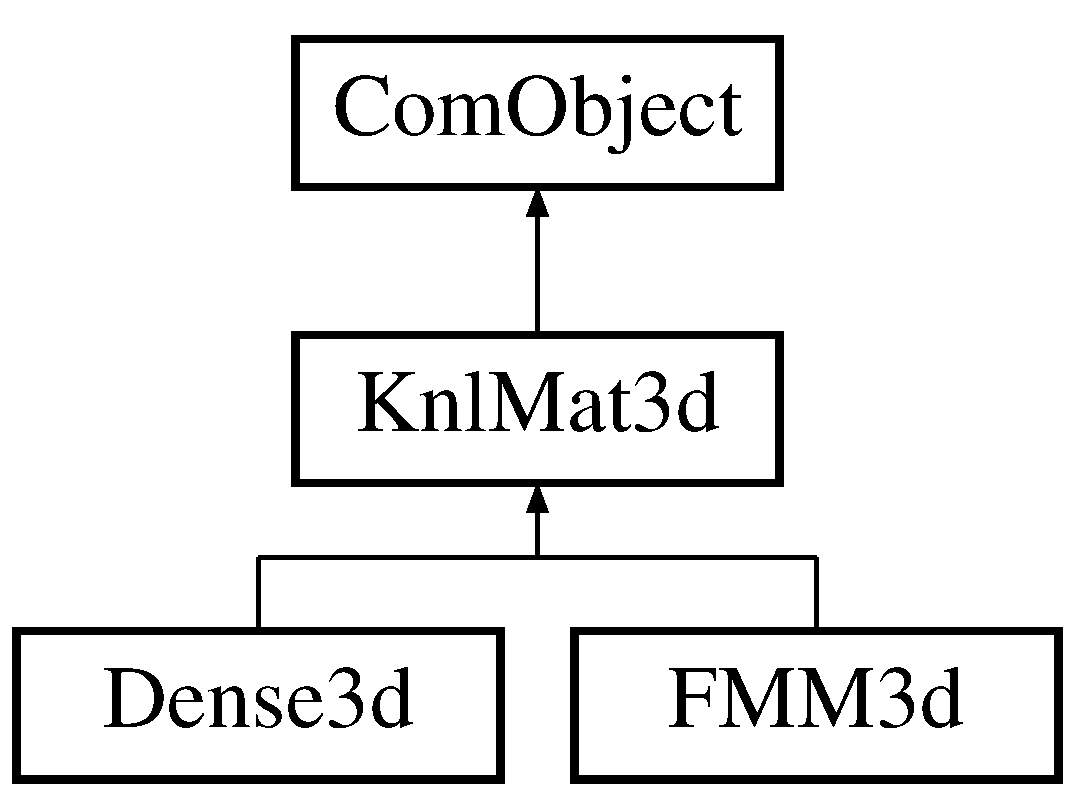
\includegraphics[height=3cm]{classKnlMat3d}
\end{center}
\end{figure}


\subsection{Detailed Description}




Definition at line 26 of file knlmat3d.hpp.\subsection*{Public Member Functions}
\begin{CompactItemize}
\item 
{\bf Knl\-Mat3d} (const string \&p)
\item 
virtual {\bf $\sim$Knl\-Mat3d} ()
\item 
Dbl\-Num\-Mat $\ast$\& {\bf src\-Pos} ()
\item 
Dbl\-Num\-Mat $\ast$\& {\bf src\-Nor} ()
\item 
Dbl\-Num\-Mat $\ast$\& {\bf trg\-Pos} ()
\item 
{\bf Kernel3d} \& {\bf knl} ()
\item 
virtual int {\bf setup} (map$<$ string, string $>$ \&)=0
\item 
virtual int {\bf evaluate} (const Dbl\-Num\-Vec \&src\-Den, Dbl\-Num\-Vec \&trg\-Val)=0
\item 
int {\bf dim} ()
\item 
int {\bf src\-DOF} ()
\item 
int {\bf trg\-DOF} ()
\end{CompactItemize}
\subsection*{Protected Attributes}
\begin{CompactItemize}
\item 
Dbl\-Num\-Mat $\ast$ {\bf \_\-src\-Pos}
\item 
Dbl\-Num\-Mat $\ast$ {\bf \_\-src\-Nor}
\item 
Dbl\-Num\-Mat $\ast$ {\bf \_\-trg\-Pos}
\item 
{\bf Kernel3d} {\bf \_\-knl}
\end{CompactItemize}


\subsection{Constructor \& Destructor Documentation}
\index{KnlMat3d@{Knl\-Mat3d}!KnlMat3d@{KnlMat3d}}
\index{KnlMat3d@{KnlMat3d}!KnlMat3d@{Knl\-Mat3d}}
\subsubsection{\setlength{\rightskip}{0pt plus 5cm}Knl\-Mat3d::Knl\-Mat3d (const string \& {\em p})\hspace{0.3cm}{\tt  [inline]}}\label{classKnlMat3d_e5c3a44fa56c9abf153bdcd2fd4acca6_e5c3a44fa56c9abf153bdcd2fd4acca6}




Definition at line 39 of file knlmat3d.hpp.

\footnotesize\begin{verbatim}39 :  ComObject(p), _srcPos(NULL), _srcNor(NULL), _trgPos(NULL) {;}
\end{verbatim}\normalsize 


\index{KnlMat3d@{Knl\-Mat3d}!~KnlMat3d@{$\sim$KnlMat3d}}
\index{~KnlMat3d@{$\sim$KnlMat3d}!KnlMat3d@{Knl\-Mat3d}}
\subsubsection{\setlength{\rightskip}{0pt plus 5cm}virtual Knl\-Mat3d::$\sim$Knl\-Mat3d ()\hspace{0.3cm}{\tt  [inline, virtual]}}\label{classKnlMat3d_41844e50417d0e54dd36950b66babb7f_41844e50417d0e54dd36950b66babb7f}




Definition at line 40 of file knlmat3d.hpp.

\footnotesize\begin{verbatim}40 { }
\end{verbatim}\normalsize 




\subsection{Member Function Documentation}
\index{KnlMat3d@{Knl\-Mat3d}!dim@{dim}}
\index{dim@{dim}!KnlMat3d@{Knl\-Mat3d}}
\subsubsection{\setlength{\rightskip}{0pt plus 5cm}int Knl\-Mat3d::dim ()\hspace{0.3cm}{\tt  [inline]}}\label{classKnlMat3d_e3f9953141ca7d7525b58c0ff1ef6b1f_e3f9953141ca7d7525b58c0ff1ef6b1f}


return dimension of the kernel matrix/fmm, set to 3 

Definition at line 57 of file knlmat3d.hpp.

Referenced by FMM3d::check(), Dense3d::evaluate(), Dense3d::setup(), FMM3d::src\-Data(), FMM3d::src\-Exa\-Nor(), FMM3d::src\-Exa\-Pos(), FMM3d::trg\-Data(), and FMM3d::trg\-Exa\-Pos().

\footnotesize\begin{verbatim}57 { return 3; }
\end{verbatim}\normalsize 


\index{KnlMat3d@{Knl\-Mat3d}!evaluate@{evaluate}}
\index{evaluate@{evaluate}!KnlMat3d@{Knl\-Mat3d}}
\subsubsection{\setlength{\rightskip}{0pt plus 5cm}virtual int Knl\-Mat3d::evaluate (const Dbl\-Num\-Vec \& {\em src\-Den}, Dbl\-Num\-Vec \& {\em trg\-Val})\hspace{0.3cm}{\tt  [pure virtual]}}\label{classKnlMat3d_fcf3de1e6ce4ee024ef0d320363bd920_fcf3de1e6ce4ee024ef0d320363bd920}


Virtual evaluation function 

Implemented in {\bf Dense3d} {\rm (p.\,\pageref{classDense3d_3d2ce8cfb3d9632d6b69352f1bb5eda2_3d2ce8cfb3d9632d6b69352f1bb5eda2})}, and {\bf FMM3d} {\rm (p.\,\pageref{classFMM3d_3d2ce8cfb3d9632d6b69352f1bb5eda2_3d2ce8cfb3d9632d6b69352f1bb5eda2})}.\index{KnlMat3d@{Knl\-Mat3d}!knl@{knl}}
\index{knl@{knl}!KnlMat3d@{Knl\-Mat3d}}
\subsubsection{\setlength{\rightskip}{0pt plus 5cm}{\bf Kernel3d}\& Knl\-Mat3d::knl ()\hspace{0.3cm}{\tt  [inline]}}\label{classKnlMat3d_d01911fc223ab4bc9604db12f942194e_d01911fc223ab4bc9604db12f942194e}


return kernel 

Definition at line 49 of file knlmat3d.hpp.

References \_\-knl.

\footnotesize\begin{verbatim}49 { return _knl; }
\end{verbatim}\normalsize 


\index{KnlMat3d@{Knl\-Mat3d}!setup@{setup}}
\index{setup@{setup}!KnlMat3d@{Knl\-Mat3d}}
\subsubsection{\setlength{\rightskip}{0pt plus 5cm}virtual int Knl\-Mat3d::setup (map$<$ string, string $>$ \&)\hspace{0.3cm}{\tt  [pure virtual]}}\label{classKnlMat3d_24cbbecf677cd909a522d252feebf2c6_24cbbecf677cd909a522d252feebf2c6}


Virtual setup function 

Implemented in {\bf Dense3d} {\rm (p.\,\pageref{classDense3d_6c9d66eef2ad01ccfea65cb116bf5726_6c9d66eef2ad01ccfea65cb116bf5726})}, and {\bf FMM3d} {\rm (p.\,\pageref{classFMM3d_d134e155a30bcbea9ad038ffcd737ddc_d134e155a30bcbea9ad038ffcd737ddc})}.\index{KnlMat3d@{Knl\-Mat3d}!srcDOF@{srcDOF}}
\index{srcDOF@{srcDOF}!KnlMat3d@{Knl\-Mat3d}}
\subsubsection{\setlength{\rightskip}{0pt plus 5cm}int Knl\-Mat3d::src\-DOF ()\hspace{0.3cm}{\tt  [inline]}}\label{classKnlMat3d_6b422ba557bb24eff82ac7125e206568_6b422ba557bb24eff82ac7125e206568}


return source degrees of freedom 

Definition at line 59 of file knlmat3d.hpp.

References \_\-knl, and Kernel3d::src\-DOF().

Referenced by FMM3d::check(), FMM3d::evaluate(), Dense3d::evaluate(), FMM3d::src\-Data(), and FMM3d::src\-Exa\-Den().

\footnotesize\begin{verbatim}59 { return _knl.srcDOF(); }
\end{verbatim}\normalsize 


\index{KnlMat3d@{Knl\-Mat3d}!srcNor@{srcNor}}
\index{srcNor@{srcNor}!KnlMat3d@{Knl\-Mat3d}}
\subsubsection{\setlength{\rightskip}{0pt plus 5cm}Dbl\-Num\-Mat$\ast$\& Knl\-Mat3d::src\-Nor ()\hspace{0.3cm}{\tt  [inline]}}\label{classKnlMat3d_bba2c6a917421951f1fbe8f69b9a135b_bba2c6a917421951f1fbe8f69b9a135b}


return source normals 

Definition at line 45 of file knlmat3d.hpp.

References \_\-src\-Nor.

\footnotesize\begin{verbatim}45 { return _srcNor; }
\end{verbatim}\normalsize 


\index{KnlMat3d@{Knl\-Mat3d}!srcPos@{srcPos}}
\index{srcPos@{srcPos}!KnlMat3d@{Knl\-Mat3d}}
\subsubsection{\setlength{\rightskip}{0pt plus 5cm}Dbl\-Num\-Mat$\ast$\& Knl\-Mat3d::src\-Pos ()\hspace{0.3cm}{\tt  [inline]}}\label{classKnlMat3d_caa1dae06f56964efa0f778b696dce61_caa1dae06f56964efa0f778b696dce61}


return source positions 

Definition at line 43 of file knlmat3d.hpp.

References \_\-src\-Pos.

\footnotesize\begin{verbatim}43 { return _srcPos; }
\end{verbatim}\normalsize 


\index{KnlMat3d@{Knl\-Mat3d}!trgDOF@{trgDOF}}
\index{trgDOF@{trgDOF}!KnlMat3d@{Knl\-Mat3d}}
\subsubsection{\setlength{\rightskip}{0pt plus 5cm}int Knl\-Mat3d::trg\-DOF ()\hspace{0.3cm}{\tt  [inline]}}\label{classKnlMat3d_ea43c1f768349e86110e4e2d06e38d10_ea43c1f768349e86110e4e2d06e38d10}


return target degrees of freedom 

Definition at line 61 of file knlmat3d.hpp.

References \_\-knl, and Kernel3d::trg\-DOF().

Referenced by FMM3d::check(), FMM3d::evaluate(), Dense3d::evaluate(), FMM3d::trg\-Data(), and FMM3d::trg\-Exa\-Val().

\footnotesize\begin{verbatim}61 { return _knl.trgDOF(); }
\end{verbatim}\normalsize 


\index{KnlMat3d@{Knl\-Mat3d}!trgPos@{trgPos}}
\index{trgPos@{trgPos}!KnlMat3d@{Knl\-Mat3d}}
\subsubsection{\setlength{\rightskip}{0pt plus 5cm}Dbl\-Num\-Mat$\ast$\& Knl\-Mat3d::trg\-Pos ()\hspace{0.3cm}{\tt  [inline]}}\label{classKnlMat3d_7dc770563c182703b1986abb06c6dbbd_7dc770563c182703b1986abb06c6dbbd}


return target positions 

Definition at line 47 of file knlmat3d.hpp.

References \_\-trg\-Pos.

\footnotesize\begin{verbatim}47 { return _trgPos; }
\end{verbatim}\normalsize 




\subsection{Member Data Documentation}
\index{KnlMat3d@{Knl\-Mat3d}!_knl@{\_\-knl}}
\index{_knl@{\_\-knl}!KnlMat3d@{Knl\-Mat3d}}
\subsubsection{\setlength{\rightskip}{0pt plus 5cm}{\bf Kernel3d} {\bf Knl\-Mat3d::\_\-knl}\hspace{0.3cm}{\tt  [protected]}}\label{classKnlMat3d_cb56a4f532a89bc1a51ee17c2434a106_cb56a4f532a89bc1a51ee17c2434a106}


Kernel. See {\bf kernel3d.hpp}{\rm (p.\,\pageref{kernel3d_8hpp})} and {\bf kernel3d.cpp}{\rm (p.\,\pageref{kernel3d_8cpp})} 

Definition at line 37 of file knlmat3d.hpp.

Referenced by Dense3d::evaluate(), knl(), src\-DOF(), FMM3d::Src\-Equ2Dwn\-Chk\_\-dgemv(), FMM3d::Src\-Equ2Trg\-Chk\_\-dgemv(), FMM3d::Src\-Equ2Upw\-Chk\_\-dgemv(), and trg\-DOF().\index{KnlMat3d@{Knl\-Mat3d}!_srcNor@{\_\-srcNor}}
\index{_srcNor@{\_\-srcNor}!KnlMat3d@{Knl\-Mat3d}}
\subsubsection{\setlength{\rightskip}{0pt plus 5cm}Dbl\-Num\-Mat$\ast$ {\bf Knl\-Mat3d::\_\-src\-Nor}\hspace{0.3cm}{\tt  [protected]}}\label{classKnlMat3d_bbeec6db21041e1b277f4755f21047dd_bbeec6db21041e1b277f4755f21047dd}


source normal 

Definition at line 33 of file knlmat3d.hpp.

Referenced by Dense3d::evaluate(), Dense3d::setup(), and src\-Nor().\index{KnlMat3d@{Knl\-Mat3d}!_srcPos@{\_\-srcPos}}
\index{_srcPos@{\_\-srcPos}!KnlMat3d@{Knl\-Mat3d}}
\subsubsection{\setlength{\rightskip}{0pt plus 5cm}Dbl\-Num\-Mat$\ast$ {\bf Knl\-Mat3d::\_\-src\-Pos}\hspace{0.3cm}{\tt  [protected]}}\label{classKnlMat3d_f66b814fdf8eb17df56ff5ff27a368da_f66b814fdf8eb17df56ff5ff27a368da}


source positions 

Definition at line 31 of file knlmat3d.hpp.

Referenced by FMM3d::check(), Dense3d::evaluate(), Dense3d::setup(), and src\-Pos().\index{KnlMat3d@{Knl\-Mat3d}!_trgPos@{\_\-trgPos}}
\index{_trgPos@{\_\-trgPos}!KnlMat3d@{Knl\-Mat3d}}
\subsubsection{\setlength{\rightskip}{0pt plus 5cm}Dbl\-Num\-Mat$\ast$ {\bf Knl\-Mat3d::\_\-trg\-Pos}\hspace{0.3cm}{\tt  [protected]}}\label{classKnlMat3d_a1b44c7c6fd0a38be167c34537b1a508_a1b44c7c6fd0a38be167c34537b1a508}


target position 

Definition at line 35 of file knlmat3d.hpp.

Referenced by FMM3d::check(), Dense3d::setup(), and trg\-Pos().

The documentation for this class was generated from the following file:\begin{CompactItemize}
\item 
fmm3d/{\bf knlmat3d.hpp}\end{CompactItemize}
